\documentclass[12pt]{article}
\usepackage{../../format}
\lhead{A Level Physics}
\setcounter{secnumdepth}{5}
\usepackage[english]{babel}

\makeatletter
\renewcommand{\paragraph}{\@startsection{paragraph}{4}{0ex}%
    {-3.25ex plus -1ex minus -0.2ex}%
    {1.5ex plus 0.2ex}%
    {\normalfont\normalsize\bfseries}}
\makeatother

\usetikzlibrary{decorations.pathmorphing,arrows}

\pgfkeys{/pgfplots/Axis Style/.style={
    width=13.5cm, height=10cm,
    axis x line=center, 
    axis y line=middle, 
    samples=100,
    ymin=-1.2, ymax=1.2,
    xmin=0, xmax=13.0,
    domain=-4*pi:4*pi
}}

\pgfkeys{/pgfplots/Stationary Wave/.style={
    width=13.5cm, height=5cm,
    axis x line=center, 
    axis y line=middle, 
    samples=100,
    ymin=-1.2, ymax=1.2,
    xmin=0, xmax=13.0,
    domain=-4*pi:4*pi
}}

\pgfkeys{/pgfplots/Axis Style 2/.style={
    width=13.5cm, height=5cm,
    axis x line=center, 
    axis y line=middle, 
    samples=100,
    ymin=-1.5, ymax=1.5,
    xmin=0, xmax=14.0,
    domain=-4*pi:4*pi
}}


\begin{document}
\begin{center}
\underline{\huge Paper 1 Cheat Sheet}
\end{center}
\section{Measurements and their errors}
\textbf{Precision} - There is very little spread around the mean value\\
\textbf{Repeatability} - If the same experimenter repeats the investigation using the same method and equipment and obtains the same results\\
\textbf{Reproducibility} - If a different experimenter repeats the investigation, or uses a different experiment or technique, the same results are obtained\\
\textbf{Accuracy} - Close to the true value\\
{\renewcommand{\arraystretch}{2}
\begin{tabularx}{\textwidth}{|X|X|}
\hline
Combination&Operation\\
\hline
Adding or subtracting\newline $a=b+c$&Add the absolute uncertainties\newline $\Delta a=\Delta b+\Delta c$\\
\hline
Multiplying values\newline $a=b\times c$&Add the percentage uncertainties\newline $\epsilon a=\epsilon b+\epsilon c$\\
\hline
Dividing values\newline $a=\dfrac{b}{c}$&Add the percentage uncertainties\newline $\epsilon a=\epsilon b+\epsilon c$\\
\hline
Power rules\newline $a=b^c$&Multiply the percentage uncertainty by the power\newline $\epsilon a=c\times\epsilon b$\\
\hline
\end{tabularx}}
\newpage
\section{Particles and radiation}
\subsection{Constituents of the atom}
Protons and neurons in the centre, with shells of electrons around them
$$\textrm{Specific charge}=\frac{Q}{m}$$
\textbf{Isotope} - An atom with the same number of protons and electrons as an element, but a different number of neutrons
\subsection{Stable and unstable nuclei}
\subsubsection{The strong nuclear force}
\begin{tabular}{|c|c|}
\hline
$<0.5fm$&Repulsion\\
\hline
$0.5-3fm$&Attraction\\
\hline
$3fm+$&No force\\
\hline
\end{tabular}
\subsubsection{Alpha decay}
{\large
$$^A_ZX\rightarrow ^{A-4}_{Z-2}Y+^4_2\alpha$$
\subsubsection{Beta decay}
$$^A_ZX\rightarrow ^A_{Z+1}+^0_{-1}\beta+\overline{\nu}$$}
Neutrinos were hypothesised to allow for energy to be conserved in the interaction
\subsection{Particles, antiparticles and photons}
\subsubsection{Particle antiparticle pairs and their properties}
{\def\arraystretch{1.5}
\begin{tabularx}{\textwidth}{|X|X|X|}
\hline
\textbf{Property}&\textbf{Particle}&\textbf{Antiparticle}\\
\hline
Mass&x&x\\
\hline
\textcolor{red}{Charge}&x&-x\\
\hline
Rest Energy&x&x\\
\hline
\textcolor{red}{Baryon Number}&x&-x\\
\hline
\textcolor{red}{Lepton Number}&x&-x\\
\hline
\textcolor{red}{Strangeness}&x&-x\\
\hline
\end{tabularx}}
\newpage
\paragraph{Mesons}
\subparagraph{Pions(All 0 Strangeness)}
$ $\\
{\def\arraystretch{1.5}
\begin{tabularx}{\textwidth}{|X|X|}
\hline
$\pi^0$&$U\bar{U}$ or $D\bar{D}$\\
\hline
$\pi^+$&$U\bar{D}$\\
\hline
$\pi^-$&$D\bar{U}$\\
\hline
\end{tabularx}}
\subparagraph{Kaons (All strange)}
$ $\\
{\def\arraystretch{1.5}
\begin{tabularx}{\textwidth}{|X|X|}
\hline
$K^+$&$U\bar{S}$\\
\hline
$K^-$&$\bar{U}S$\\
\hline
$K^0$&$D\bar{S}$\\
\hline
$\bar{K^0}$&$\bar{D}S$\\
\hline
\end{tabularx}}
\subsubsection{The photon model of electromagnetic radiation}
A photon is a particle whose energy depends on its frequency. Formulas can be found on the data sheet to calculate this relationship
\subsubsection{Methods of annihilation and pair production}
\paragraph{Annihilation}
When a particle and an antiparticle meet, they annihilate each other, releasing two photons, with energy sum equivalent to the sum of the energy of the particle and antiparticle. This energy can be calculated from the rest energy values on the data sheet.
$$hf_{min}=E_0$$
\paragraph{Pair production}
In pair production a photon creates a particle and an antiparticle
$$hf_{min}=2E_0$$
\subsection{Particle interactions}
\subsubsection{The four fundamental interactions}
{\def\arraystretch{1.5}
\begin{tabularx}{\textwidth}{|X|X|X|X|}
\hline
\textbf{Force}&\textbf{Affects}&\textbf{Gauge Boson}&\textbf{Range}\\
\hline
Gravitational&Mass&Graviton&Infinite\\
\hline
Electromagnetic&Charge&Photon&Infinite\\
\hline
Nuclear Strong&Quarks&Gluon(Pion)&$10^{-15}$m\\
\hline
Nuclear Weak&Leptons+Quarks&$W^+,W^-,Z^0$&$10^{-18}$m\\
\hline
\end{tabularx}}
\newpage
\subsubsection{Diagrams to represent the interactions}
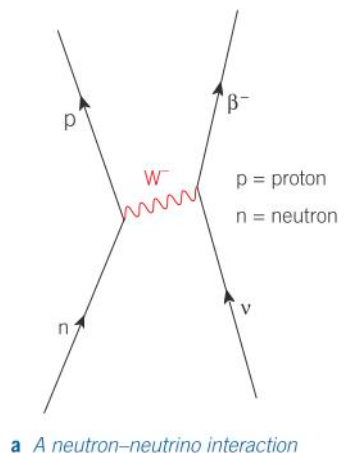
\includegraphics[width=6cm]{neutron-neutrino.png}
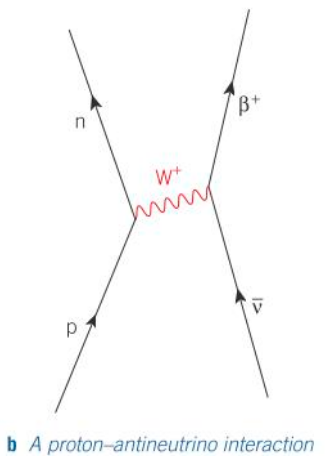
\includegraphics[width=6cm]{proton-antineutrino.png}
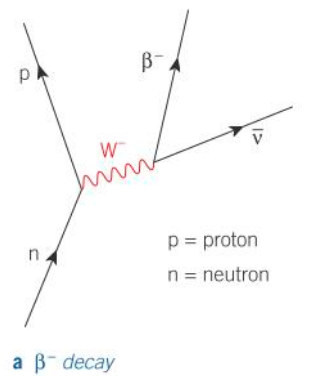
\includegraphics[width=6cm]{betaminus.png}
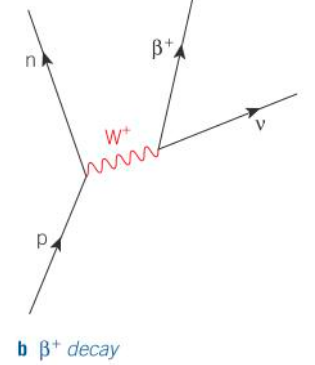
\includegraphics[width=6cm]{betaplus.png}
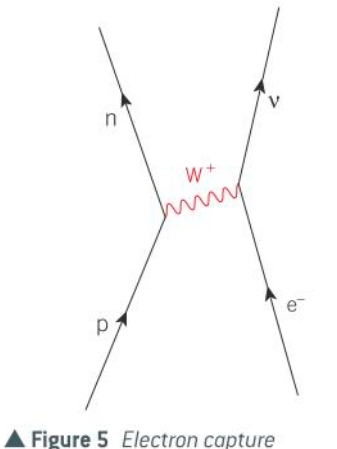
\includegraphics[width=6cm]{electron_capture.png}
\subsection{Classifications of particles}
{\renewcommand{\arraystretch}{2}
\begin{tabularx}{\textwidth}{|X|X|X|X|X|X|X|}
\hline
&\multicolumn{2}{|c|}{\centering Hadron}&\multicolumn{4}{|c|}{\centering Lepton}\\
\cline{2-7}
&Baryon&Meson&Electron&Muon&Electron neutrino&Muon neutrino\\
\hline
What it is&3 quarks&Quark antiquark pair&&&&\\
\hline
\end{tabularx}}
\paragraph{Baryons}
\begin{itemize}
\item Baryon number is conserved during interactions
\item The proton is the only stable baryon, all other baryons decay to it
\end{itemize}
\paragraph{Kaons and pions}
Kaons (K mesons) decay into Pions($\pi$ mesons), they decay by the weak interaction, so strangeness need not be conserved
$$K^+\rightarrow \mu^++\nu_\mu$$
$$K^+\rightarrow \pi^++\pi^0$$
$$K^-\rightarrow \mu^-+\overline{\nu_\mu}$$
$$K^-\rightarrow \pi^-+\pi^0$$
$$K^-\rightarrow \pi^0+\mu^-+\overline{\nu_\mu}$$
\paragraph{Leptons}
Lepton number is conserved in an interaction, muons decay into electrons
$$\mu^-\rightarrow e^-+\overline{\nu_e}+\nu_\mu$$
$$\mu^+\rightarrow e^++\nu_e+\overline{\nu_\mu}$$
\paragraph{Strange particles}
Strange particles are produced through the strong interaction and decay through the weak interaction, this is because strangeness is conserved during the strong interaction, but not during the weak interaction.
\subsubsection{Quarks and antiquarks}
Differences between quarks and antiquarks
\begin{itemize}
\item Opposite strangeness
\item Opposite charge
\item Opposite strangeness
\end{itemize}
\paragraph{Quark compositions}
\begin{itemize}
\item Proton -UUD
\item Neutron - DUD
\item Pion - Not strange, sign indicates charge
\item Kaon - Strange, sign indicates charge
\end{itemize}
\subsubsection{Applications of conservation laws}
Changes of quark nature
\begin{itemize}
\item $\beta^-$, down $\rightarrow$ up
\item $\beta^+$, up $\rightarrow$ down
\end{itemize}
\begin{center}
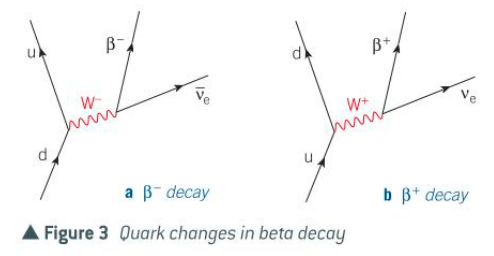
\includegraphics[width=10cm]{quark_beta.png}
\end{center}
In all interactions, energy and momentum must be conserved
\subsection{Electromagnetic radiation and quantum phenomena}
\subsubsection{The photoelectric effect}
\textbf{Photoelectric effect} - The emission of electrons from a metal surface when the surface is illuminated by a light of frequency greater than a minimum value known as the threshold frequency
\paragraph{Threshold frequency}
Because the energy of a photon is proportional to its frequency ($E=hf$), a minimum frequency must be reached so that the electrons have sufficient energy to escape the surface
\paragraph{Work function and stopping potential}
\textbf{Work function} - The minimum amount of energy needed by an electron to escape from a metal surface\\
\textbf{Stopping potential} - The potential difference required to stop an electron
\paragraph{The photoelectric equation}
$$hf=\phi+E_{K(Max)}$$
$hf$ is the energy of the incident photon\\
$\phi$ is the work function\\
$E_{K(max)}$ is the maximum kinetic energy\\
Electrons emitted will have a range of kinetic energies, depending how much work is done to escape the metal\\
\begin{tikzpicture}
\begin{axis}[axis lines=middle,scale=0.8,ylabel = KE,xlabel=Frequency,ylabel style={rotate=90,anchor=south},xlabel style={anchor=south},xmin=0,xmax=7,ymin=-5,ymax=7,xtick={2},xticklabels={$F_0$},ytick={-2},yticklabels={$-\Phi$}
]
\addplot[color=black,domain=0:7]{x-2};
\end{axis}
\end{tikzpicture}\\
The gradient of the line is Planck's constant
\subsubsection{Collisions of electrons with atoms}
\paragraph{Ionisation and excitation}
\textbf{Ion} - A charged atom\\
\textbf{Ionisation} - The process of creating ions\\
\textbf{Excitation} - The process in which an atom absorbs energy without becoming ionised as a result of an electron inside an atom moving from an inner shell to an outer shell
\paragraph{The fluorescent tube}
\begin{itemize}
\item Ionisation and excitation of the mercury atoms as they collide with each other and the electrons in the tube
\item The mercury atoms emit visible and ultraviolet photons when they de excite
\item The ultraviolet photons are absorbed by the atoms in the fluorescent coating, causing them to excite
\item The atoms in the coating de excite, emitting visible light
\end{itemize}
\paragraph{The electron volt}
\textbf{Electron volt} - The work done when an electron is moved through a P.D. of 1V
\subsubsection{Energy levels and photon emission}
\paragraph{Line spectra}
Light is emitted from an atom when the electrons in it de-excite. Because the line spectra are discrete, this suggests that only certain changes in energies are possible in the atom, implying discrete energy levels
$$hf=E_1-E_2$$
Energies given in joules
\subsubsection{Wave particle duality}
\paragraph{Electron diffraction}
When electrons are fired at a slit, they exhibit the same behaviour as light does, implying that particles can posses wave properties.
\paragraph{The photoelectric effect}
Because there is a threshold frequency for the photoelectric effect, light must have a particle nature, where one particle provides the energy to release the electron. If it had a wave nature, given enough time, an electron would be released, regardless of frequency
\paragraph{The de Broglie Wavelength}
$$\lambda=\frac{h}{p}=\frac{h}{mv}$$
This causes the amount of diffraction to change based on the momentum of the particle, the greater the momentum, the smaller the wavelength, and so the less diffraction.
\section{Waves}
\subsection{Progressive and stationary waves}
\subsubsection{Progressive waves}
\textbf{Amplitude} - The maximum displacement of a vibrating particle\\
\textbf{Frequency} - The number of cycles of a wave that pass a point per second\\
\textbf{Period} - The time for one complete cycle of a wave to pass a point\\
\textbf{Wavelength} - The least distance between two vibrating particles with the same displacement and velocity at the same time\\
\textbf{Phase} - The position of a point in time on a waveform cycle\\
\textbf{Phase difference} - The fraction of a cycle between the vibrations of two vibrating particles
\subsubsection{Longitudinal and transverse waves}
\paragraph{Transverse wave}
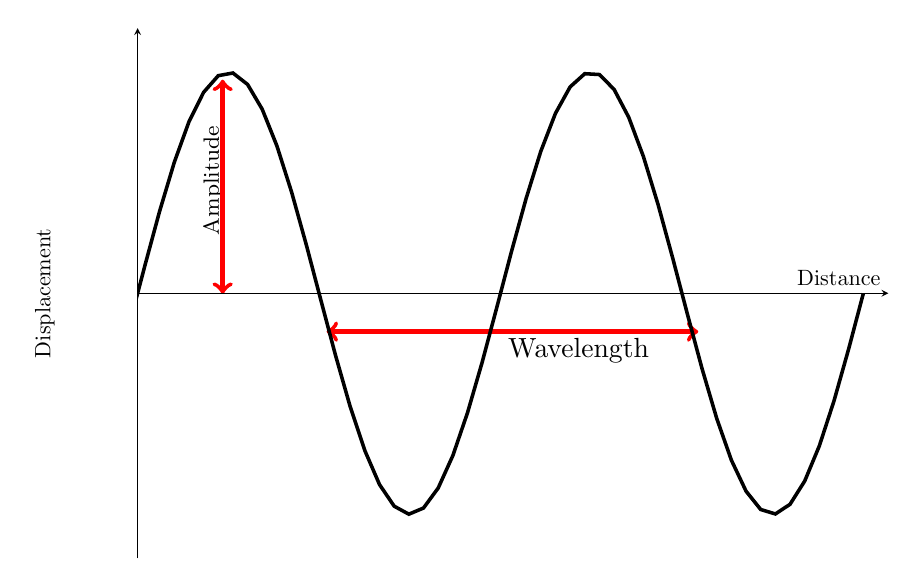
\begin{tikzpicture}[scale=0.8]
\tikzstyle{vlabel} = [fill=white,font=\footnotesize,inner sep=1pt,rotate=90]
\tikzstyle{hlabel} = [fill=white,font=\normalsize,inner sep=1pt]
\node[vlabel] at (1.2,6) {Amplitude};
\draw[arrows=<->,red,ultra thick](1.35,4.2)--(1.35,7.6);
\node[hlabel] at (7,3.3) {Wavelength};
\draw[arrows=<->,red,ultra thick](3,3.6)--(8.9,3.6);

\begin{axis}[
    Axis Style,
    y label style={at={(axis description cs:-0.1,.5)},rotate=90,anchor=south},
    ylabel = {Displacement},
    xlabel= {Distance},
    ticks=none
]
\addplot [mark=none, ultra thick, black] {sin(deg(x))};
\end{axis}
\end{tikzpicture}
\\
\\
Wave direction and energy are perpendicular
\paragraph{Longitudinal wave}
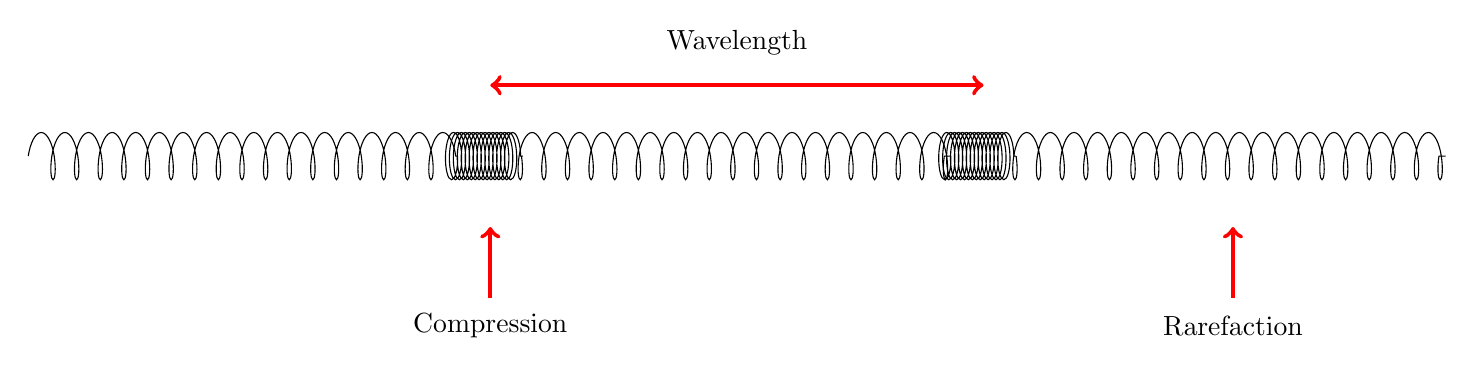
\begin{tikzpicture}[decoration={coil},scale=1.8]
\tikzstyle{hlabel} = [fill=white,font=\normalsize,inner sep=1pt]
\node[hlabel] at (5,0.8) {Wavelength};

\draw[arrows=<->,red,ultra thick](3.26,0.5)--(6.74,0.5);
\draw[arrows=->,red,ultra thick](3.26,-1)--(3.26,-0.5);
\draw[arrows=->,red,ultra thick](8.5,-1)--(8.5,-0.5);
\node[hlabel] at (3.26,-1.2) {Compression};
\node[hlabel] at (8.5,-1.2) {Rarefaction};
\draw[decorate, decoration={aspect=0.3, segment length=3mm, amplitude=3mm}] (0,0) --(3.03,0);
\draw[decorate, decoration={aspect=0.3, segment length=0.5mm, amplitude=-3mm}] (3.03,0) -- (3.49,0); 
\draw[decorate, decoration={aspect=0.3, segment length=3mm, amplitude=-3mm}] (3.48,0) -- (6.51,0);
\draw[decorate, decoration={aspect=0.3, segment length=0.5mm, amplitude=-3mm}] (6.51,0) -- (6.97,0);
\draw[decorate, decoration={aspect=0.3, segment length=3mm, amplitude=-3mm}] (6.97,0) -- (10,0);
\end{tikzpicture}\\
Wave direction and energy are parallel
\paragraph{Polarisation}
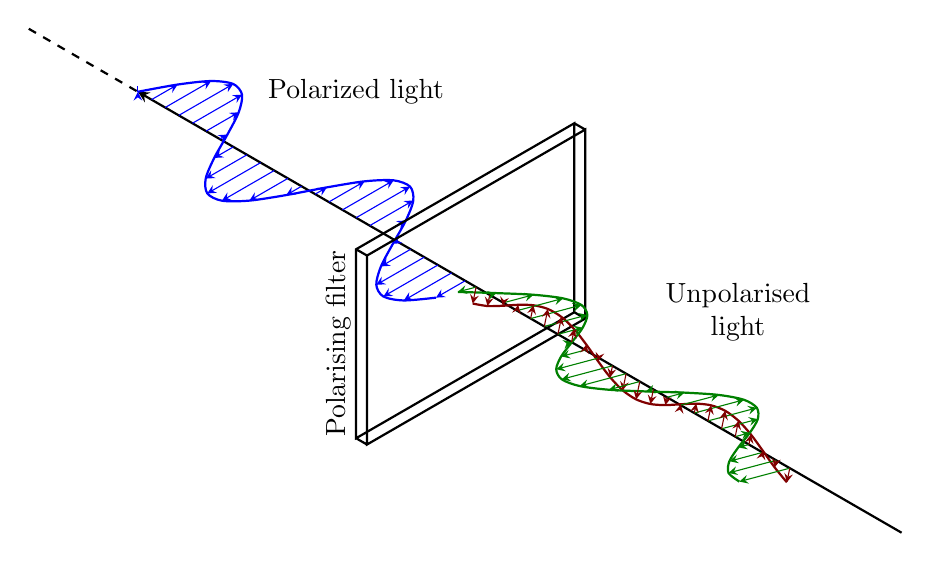
\begin{tikzpicture}[x={(0.866cm,-0.5cm)}, y={(0.866cm,0.5cm)}, z={(0cm,1cm)}, scale=.8,
    %Option for nice arrows
    >=stealth, %
    inner sep=0pt, outer sep=2pt,%
    axis/.style={thick,<-},
    wave/.style={thick,color=#1,smooth},
    polaroid/.style={fill=black!60!white, opacity=0.3},
]
    % Colors
    \colorlet{darkgreen}{green!50!black}
    \colorlet{lightgreen}{green!80!black}
    \colorlet{darkred}{red!50!black}
    \colorlet{lightred}{red!80!black}

    % Frame
    \coordinate (O) at (0, 0, 0);
    \draw[axis] (O) -- +(14, 0,   0);
    \draw[thick,dashed] (-2,0,0) -- (0,0,0);

    % Electric field vectors
    \draw[wave=blue, variable=\x,samples at={0,0.25,...,6}]
        plot (\x,{sin(2*\x r)},0);
    %Polarized light between polaroid and thin section
    \foreach \x in{0, 0.25,...,6}
        \draw[color=blue,->] (\x,0,0) -- (\x,{sin(2*\x r)},0);

    \draw (3,1,1) node [text width=2.5cm, text centered]{Polarized light};

    %Crystal thin section
    \begin{scope}[thick]
        \draw (6,-2,-1.5) -- (6,-2,1.5) node [above, sloped, midway]{Polarising filter}
                -- (6, 2, 1.5) -- (6, 2, -1.5) -- cycle % First face
            (6,  -2, -1.5) -- (6.2, -2,-1.5)
            (6,   2, -1.5) -- (6.2,  2,-1.5)
            (6,  -2,  1.5) -- (6.2, -2, 1.5)
            (6,   2,  1.5) -- (6.2,  2, 1.5)
            (6.2,-2, -1.5) -- (6.2, -2, 1.5) -- (6.2, 2, 1.5) 
                -- (6.2, 2, -1.5) -- cycle; % Second face
    \end{scope}

    %Rays leaving thin section
    \draw[wave=darkred,   variable=\x, samples at={6.2,6.45,...,12}] 
        plot (\x, {0.26*0.26*sin(2*(\x-0.5) r)},  {0.966*0.26*sin(2*(\x-0.5) r)});  %n'g-oriented ray
    \draw[wave=darkgreen, variable=\x, samples at={6.2,6.45,...,12}]
        plot (\x, {0.966*0.966*sin(2*(\x-0.1) r)},{-0.26*0.966*sin(2*(\x-0.1) r)}); %n'p-oriented ray
    \draw (10,1,1) node [text width=2.5cm, text centered] {Unpolarised light};

    \foreach \x in{6.2,6.45,...,12} {
        \draw[color=darkgreen, ->] (\x, 0, 0) --
            (\x, {0.966*0.966*sin(2*(\x-0.1) r)}, {-0.26*0.966*sin(2*(\x-0.1) r)});
        \draw[color=darkred,   ->] (\x, 0, 0) --
            (\x, {0.26*0.26*sin(2*(\x-0.5) r)}, {0.966*0.26*sin(2*(\x-0.5) r)});
            }
\end{tikzpicture}\\
Polarised light all travels in the same direction\\
Unpolarised light travels in all directions\\
Unpolarised light can be polarised using a polarising filter which contains stripes, only allowing one direction of light through\\
\textbf{Only transverse waves can be polarised}
\subsubsection{Principle of superposition of waves and formation of stationary waves}
Stationary waves are formed when a wave collides with itself after reflection\\
\\
\\
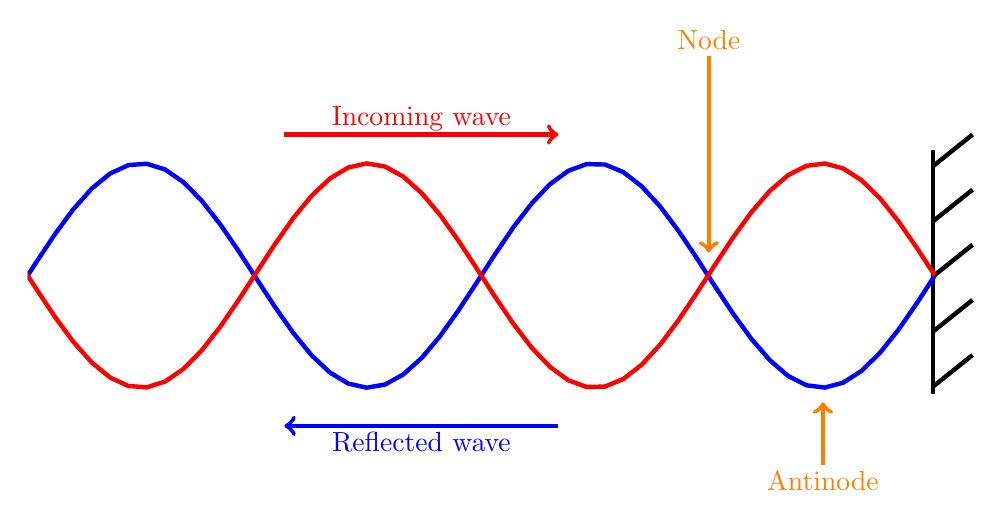
\begin{tikzpicture}
\draw[black,ultra thick] (11.5,0.2) -- ++(0,3.1);
\draw[black,ultra thick] (11.5,0.3) -- (12,0.7);
\draw[black,ultra thick] (11.5,1) -- ++(0.5,0.4);
\draw[black,ultra thick] (11.5,1.7) -- ++(0.5,0.4);
\draw[black,ultra thick] (11.5,2.4) -- ++(0.5,0.4);
\draw[black,ultra thick] (11.5,3.1) -- ++(0.5,0.4);
\tikzstyle{hlabel} = [font=\normalsize,inner sep=1pt]
\draw[arrows=->,red,ultra thick](3.26,3.5)--(6.74,3.5);
\node[hlabel,red] at (5,3.7) {Incoming wave};
\draw[arrows=<-,blue,ultra thick](3.26,-0.2)--(6.74,-0.2);
\node[hlabel,blue] at (5,-0.4) {Reflected wave};
\draw[arrows=->,orange,ultra thick](10.1,-0.7)-- ++(0,0.8);
\node[hlabel,orange] at (10.1,-0.9) {Antinode};

\draw[arrows=->,orange,ultra thick](8.65,4.5)-- ++(0,-2.5);
\node[hlabel,orange] at (8.65,4.7) {Node};



\begin{axis}[
    Stationary Wave,
    ticks=none,
    axis line style={draw=none}
]
\addplot [mark=none, ultra thick, blue] {sin(deg(x))};
\addplot [mark=none, ultra thick, red] {sin(deg(x+pi))};
\end{axis}
\end{tikzpicture}
\\
When both waves are at equilibrium there is a \textbf{node}\\
When one wave is at a maximum and one at a minimum there is an \textbf{antinode}\\
\\
\textbf{Stationary wave} - Wave pattern with nodes and antinodes formed when two or more progressive waves of the same frequency and amplitude pass through each other\\
\textbf{Node} - A fixed point in a stationary wave pattern where the amplitude is zero\\
\textbf{Antinode} - A fixed point in a stationary wave pattern where the amplitude is a maximum
\paragraph{Harmonics}
$$f_1=\frac{1}{2l}\sqrt{\frac{T}{\mu}}$$
T - String tension\\
$\mu$ - Mass/Length\\
\\
The formula for the nth harmonic is:
$$f_n=\frac{n}{2l}\sqrt{\frac{T}{\mu}}$$
\subsection{Refraction, diffraction and interference}
\subsubsection{Interference}
\textbf{Path difference} - The difference in distances from two coherent sources to an interference fringe\\
\textbf{Coherence} - Constant phase difference\\
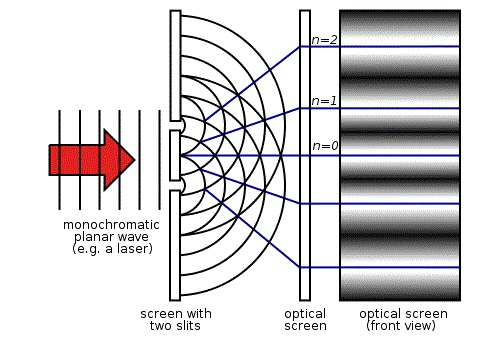
\includegraphics[width=8cm]{Interference.jpg}
$$w=\frac{\lambda D}{s}$$
w- Separation of fringes (Distance between adjacent brightest points etc)\\
$\lambda$ - Wavelength\\
D - Distance from slits to screen\\
s - Separation of the two slits\\
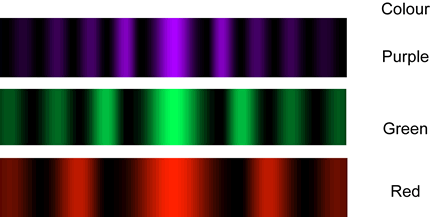
\includegraphics[width=8cm]{Diffraction_Colours.png}
\subsubsection{Diffraction}
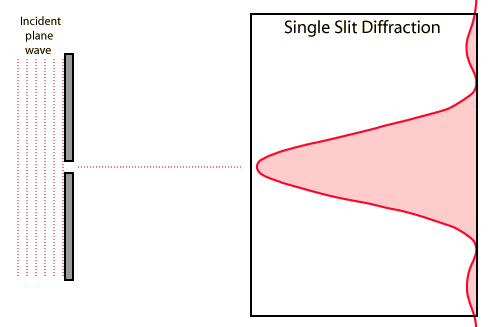
\includegraphics[width=7cm]{Diffraction.png}\\
Increasing the width of the slit causes the central maxima to get narrower, this can be remembered from the fringe spacing formula, remember the central maxima is double the width calculated using that formula though.
\paragraph{Diffraction grating equation}
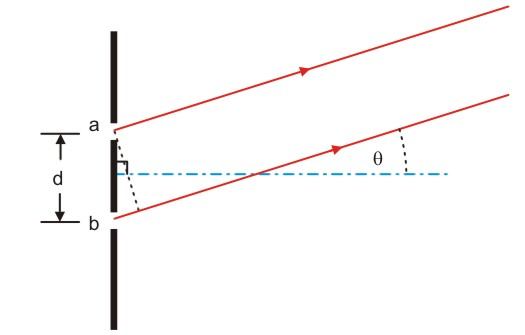
\includegraphics[width=7cm]{nlambda_1.png}\\
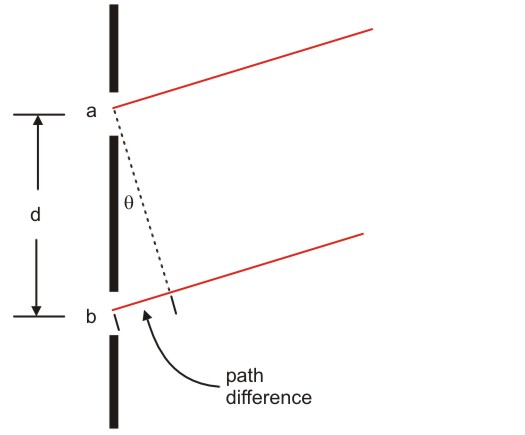
\includegraphics[width=7cm]{nlambda_2.png}\\
Path difference =$d\sin\theta$\\
$n\lambda=d\sin\theta$\\
\\
A diffraction grating can be used to analyse spectra
\subsubsection{Refraction}
\textbf{Refractive index} - $\frac{\textrm{Speed of light in free space}}{\textrm{Speed of light in that medium}}$
$$\textrm{Snell's law:} - n_1\sin\theta_1=n_2\sin\theta_2$$
$$\sin\theta_c=\frac{n_1}{n_2}$$
Total internal reflection occurs if the angle of incidence is \textbf{larger} than the critical value
\paragraph{Fibre optics}
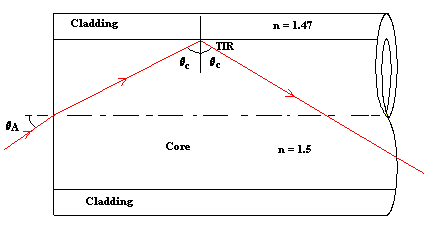
\includegraphics[width=7cm]{Fibre_Optic_1.png}\\
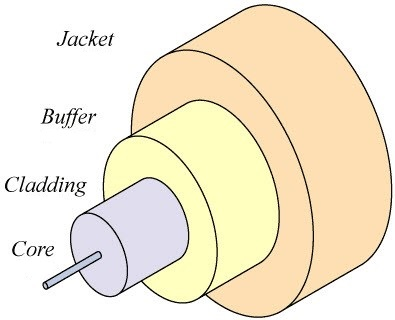
\includegraphics[width=7cm]{Fibre_Optic_2.jpg}\\
\subsubsection{Modal Dispersion}
Waves entering the fibre at different angles will reflect differently and so will have different path lengths
\subsubsection{Material Dispersion}
Different wavelengths of light enter the same but refract differently, causing a difference in path length
\section{Mechanics and materials}
\subsection{Forces, energy and momentum}
\subsubsection{Moments}
\textbf{Moment} - Force $\times$ perpendicular distance from the line of action of the force to the point\\
\textbf{Couple} - A pair of equal and opposite coplanar forces
$$\textrm{Moment of a couple}=Fd$$
Where F is one of the forces, and d is the distance between them\\
\textbf{Principle of moments} - For an object in equilibrium, the sum of clockwise moments equals the sum of anticlockwise moments\\
\textbf{Centre of mass} - The point through which a single force on the body has no turning effect
\subsubsection{Projectile motion}
\paragraph{The effect of air resistance}
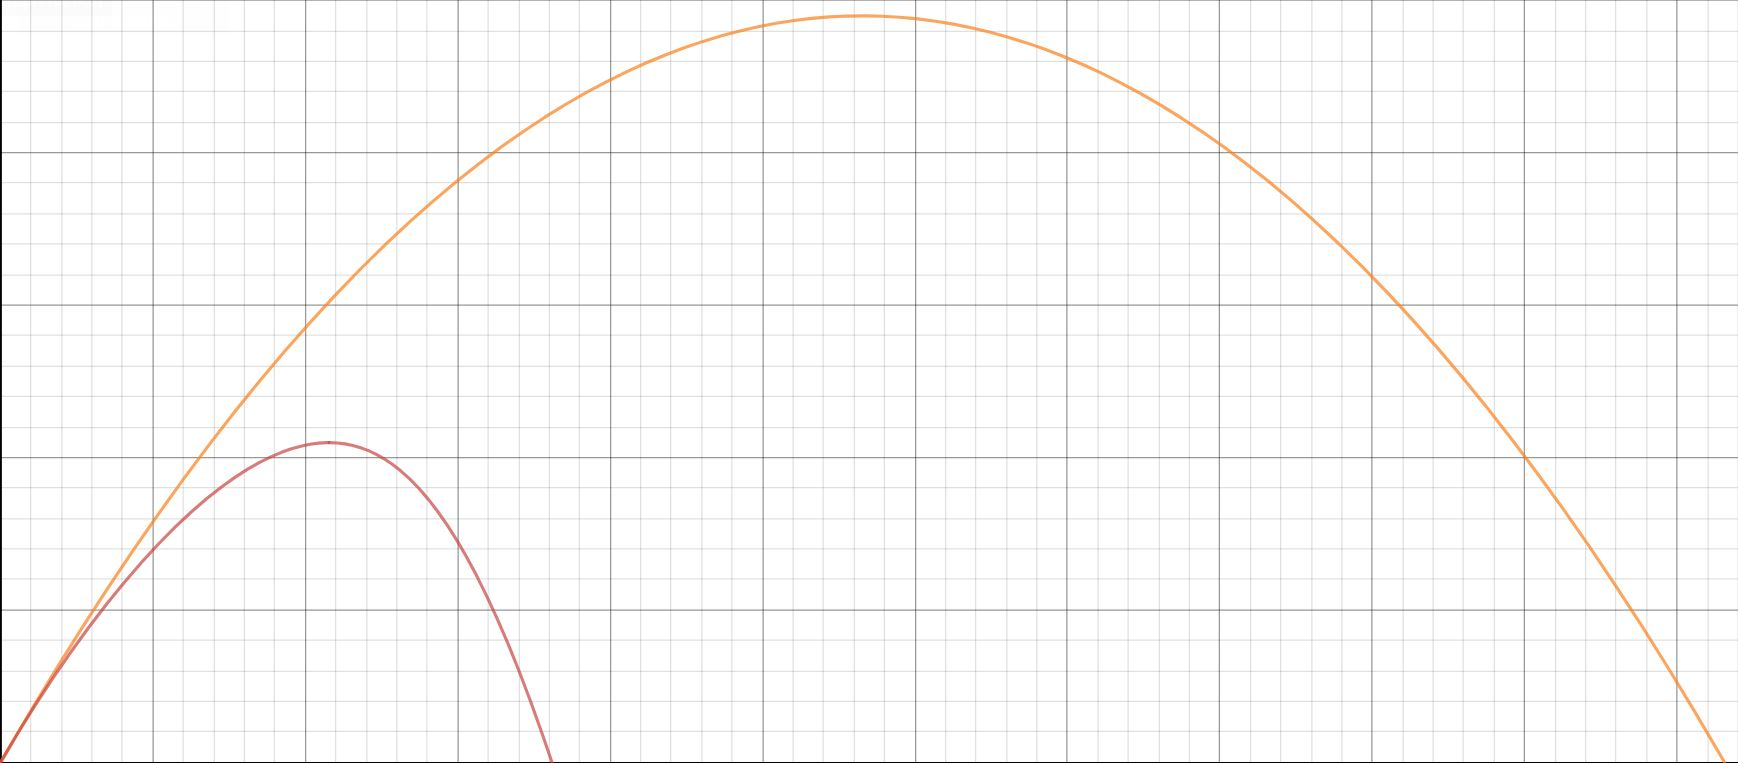
\includegraphics[scale=0.25]{Air_Resistance.JPG}\\
\textcolor{orange}{No Air Resistance}\\
\textcolor{red}{Air resistance
\begin{itemize}
\item Steeper descent
\item Peak Further Left
\item Smaller Range
\end{itemize}}
\subsubsection{Newton's laws of motion}
\textbf{1st law} - An object remains at rest or in uniform motion unless acted on by a resultant force\\
\textbf{2nd law} - $F=ma$\\
\textbf{3rd law} - Every action has an equal and opposite reaction
\subsubsection{Momentum}
\textbf{Momentum} - Mass$\times$Velocity\\
\textbf{Impulse} - Change in momentum per second\\
\textbf{Elastic collision} - No loss of kinetic energy\\
\textbf{Inelastic collision} - Loss of kinetic energy
\subsubsection{Work, energy and power}
When \textbf{work} is done \textbf{energy} is transferred
$$W=FS\cos\theta$$
\subsubsection{Conservation of energy}
\textbf{Principle of conservation of energy} - Energy cannot be created or destroyed
\subsection{Materials}
\subsubsection{Bulk properties of solids}
\textbf{Hooke's law} - Force is proportional to extension, provided the proportionality limit has not been reached\\
\textbf{Breaking stress (Ultimate tensile stress)} - Tensile stress needed to break a solid material\\
\textbf{Plastic deformation} - Deformation of a solid beyond its elastic limit\\
\textbf{Brittle} - Snaps without bending or stretching when subject to stress\\
\textbf{Fracture} - The separation of a material into two or more pieces when subject to stress\\
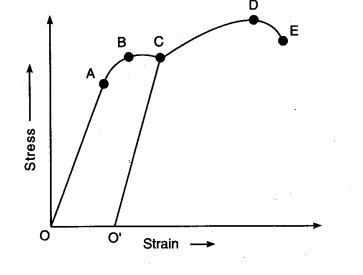
\includegraphics[width=6cm]{metal.jpg}
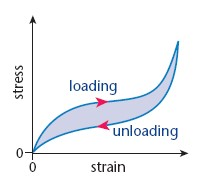
\includegraphics[width=6cm]{rubber.jpg}
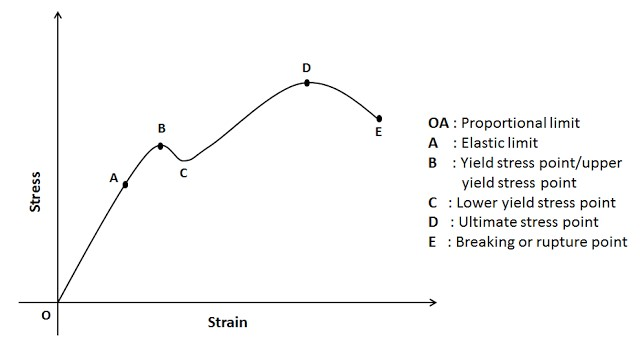
\includegraphics[width=6cm]{Stress_Strain.jpg}
\subsubsection{The Young Modulus}
\textbf{Young Modulus} - Stress/Strain assuming the limit of proportionality has not been reached
\section{Electricity}
\subsection{Current electricity}
\subsubsection{Basics of electricity}
\textbf{Current} - The rate of flow of charge\\
\textbf{Potential difference} - Work done per unit charge\\
\textbf{Resistance} - Voltage/current
\subsubsection{Current - Voltage characteristics}
\paragraph{Ohmic Conductor}
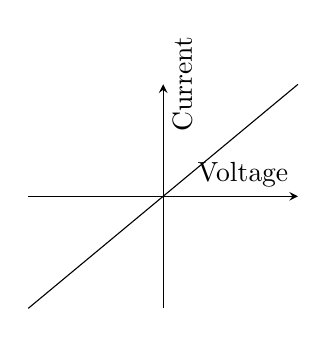
\begin{tikzpicture}
\begin{axis}[axis lines=middle, ticks=none,scale=0.5,    ylabel = Current,xlabel=Voltage,ylabel style={rotate=90}
]
\addplot[color=black]{x};
\end{axis}
\end{tikzpicture}
\paragraph{Bulb}
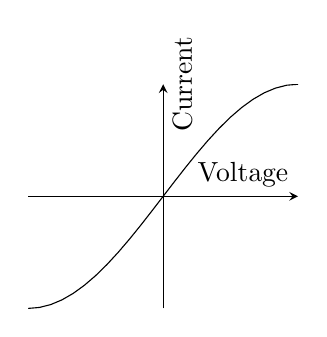
\begin{tikzpicture}
\begin{axis}[axis lines=middle, ticks=none,scale=0.5,    ylabel = Current,xlabel=Voltage,ylabel style={rotate=90}
]
\addplot[color=black,domain=-90:90]{sin(x)};
\end{axis}
\end{tikzpicture}
\paragraph{Diode}
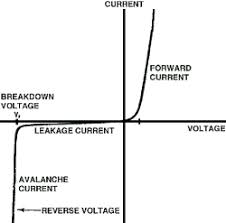
\includegraphics[width=2in]{diode.jpeg}\\
\textbf{Ohm's Law}: Current is proportional to voltage under constant physical conditions
\subsubsection{Resistivity}
\paragraph{The effect of temperature on conductors}
The lower the temperature, the less the vibration of the atoms, and resistance reduces\\
\textbf{Superconductor} - A material that has no electrical resistance\\
\textbf{Critical temperature} - The temperature below which a conductor becomes a superconductor\\
\\
Superconductors are used for very high current applications.
\subsubsection{Circuits}
\paragraph{Resistor combinations}
$$\textrm{Series}: R_T=R_1+R_2+R_3...$$
$$\textrm{Parallel}: \frac{1}{R_T}=\frac{1}{R_1}+\frac{1}{R_2}+\frac{1}{R_3}+...$$
\paragraph{Voltage in series and parallel}
Parallel: Voltage across components in parallel is the same\\
Series: The total voltage across all the components is the voltage supplied
\paragraph{Current in series and parallel}
The current entering a component or junction is the same as the current leaving the component, meaning current in series is the same for each component.\\
For parallel circuits, use voltage and resistance to calculate
\paragraph{Power}
$$P=\frac{E}{t}$$
\paragraph{Kirchoff's laws}
Current in=Current out (Conservation of charge)\\
The sum of all the voltages around the system is zero (Conservation of energy)
\subsubsection{Potential divider}
$$V_{Out}=V_{In}\frac{R_2}{R_1+R_2}$$
Potential dividers can be used with environment sensors that change their resistance based on changed to the environment to change output voltage
\subsubsection{The electromotive force and internal resistance}
\textbf{Electromotive force} - The amount of electrical energy per unit charge produced inside a source of electrical energy\\
\textbf{Internal resistance} - Resistance inside a source of electrical energy\\
\textbf{Terminal pd} - The potential difference across the terminals of a power supply\\
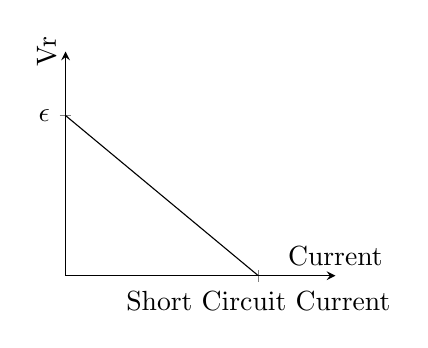
\begin{tikzpicture}
\begin{axis}[axis lines=middle,scale=0.5,    ylabel = Vr,xlabel=Current,ylabel style={rotate=90,anchor=south},xlabel style={anchor=south},xmin=0,xmax=7,ymin=0,ymax=7,xtick={5},xticklabels={Short Circuit Current},ytick={5},yticklabels={$\epsilon$}
]
\addplot[color=black,domain=0:5]{-x+5};
\end{axis}
\end{tikzpicture}
\\
The equation of this line can be derived from:
$$\epsilon=I(R+r)$$
Remember that the terminal voltage is $Ir$
\newpage
\section{Periodic motion}
\subsection{Circular motion}
As circular motion has a constant speed but a changing direction, it is implied that there is a force perpendicular to the direction of motion, and so an acceleration\\
$v$ (Velocity)- Displacement per unit time\\
$\omega$ (Angular velocity)- Angle per unit time\\
\subsection{Simple harmonic motion}
\begin{tikzpicture}
\begin{axis}[
    Axis Style 2,
    xtick={
        3.14159,6.28319,9.42478,12.56637
    },
    xticklabels={
        $\dfrac{T}{2}$,T,$\dfrac{3T}{2}$,2T
    },
    ytick={-1,1},
    yticklabels={-A,A},
    y label style={at={(axis description cs:-0.1,.5)},rotate=90,anchor=south},
    ylabel = {Displacement, x},
    xlabel= {Time, t}
]
\addplot [mark=none, ultra thick, black] {cos(deg(x))};
\end{axis}
\end{tikzpicture}
$x=Acos(\omega t)$
\\
\begin{tikzpicture}
\begin{axis}[
    Axis Style 2,
    xtick={
        3.14159,6.28319,9.42478,12.56637
    },
    xticklabels={
        $\dfrac{T}{2}$,T,$\dfrac{3T}{2}$,2T
    },
    ytick={-1,1},
    yticklabels={$-\omega A$,$\omega A$},
    y label style={at={(axis description cs:-0.1,.5)},rotate=90,anchor=south},
    ylabel = {Velocity, v},
    xlabel= {Time, t}
]
\addplot [mark=none, ultra thick, black] {-sin(deg(x))};
\end{axis}
\end{tikzpicture}
$v=-\omega A\sin(\omega t)$
\\
\begin{tikzpicture}
\begin{axis}[
    Axis Style 2,
    xtick={
        3.14159,6.28319,9.42478,12.56637
    },
    xticklabels={
        $\dfrac{T}{2}$,T,$\dfrac{3T}{2}$,2T
    },
    ytick={-1,1},
    yticklabels={$-\omega^2 A$,$\omega^2 A$},
    y label style={at={(axis description cs:-0.1,.5)},rotate=90,anchor=south},
    ylabel = {Acceleration, a},
    xlabel= {Time, t}
]
\addplot [mark=none, ultra thick, black] {-cos(deg(x))};
\end{axis}
\end{tikzpicture}
$a=-\omega^2A\cos(\omega t)$\\
\\
All these equations can be derived from the equation $x=A\cos(\omega t)$, by differentiating it with respect to time.\\
The maximum values of each of them can be found as the maximum value of cos or sin is 1
\subsection{Simple harmonic systems}
\subsubsection{Energy in SHM}
\begin{tikzpicture}
\begin{axis}[
    Axis Style 2,
    xtick={
        3.14159,6.28319
    },
    xticklabels={
        $\dfrac{T}{2}$,T
    },
    ytick={1},
    yticklabels={$\frac{1}{2}m\omega^2A^2$},
    y label style={at={(axis description cs:-0,.25)},rotate=90,anchor=south},
    ylabel = {Energy/J},
    xlabel= {Time, t},
    x label style={at={(axis description cs:1.12,0)},anchor=east},
    xmax=6.28319,
    ymin=0
]
\addplot [mark=none, ultra thick, black,samples=200] {(cos(deg(x)))^2};
\addplot [mark=none, ultra thick, red,samples=200] {(sin(deg(x)))^2};
\end{axis}
\end{tikzpicture}
\\
Red - Kinetic Energy\\
Black - Gravitational potential energy\\
\\
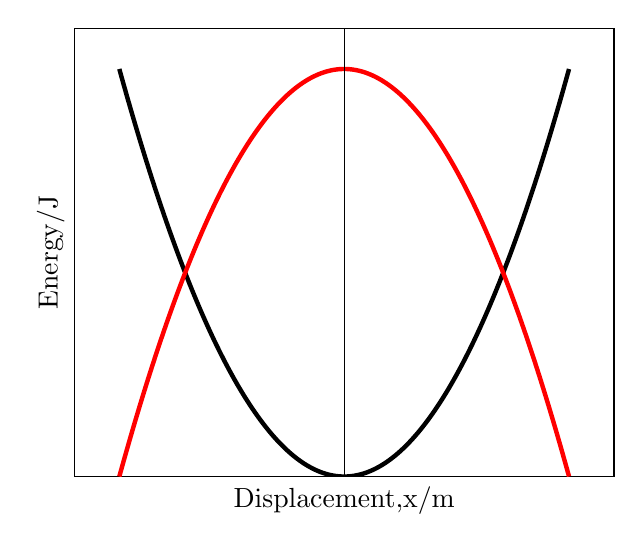
\begin{tikzpicture}
\begin{axis}[ymin=0,ticks=none,xlabel={Displacement,x/m},ylabel={Energy/J}]
\addplot [mark=none, ultra thick, black,samples=200] {x^2};
\addplot [mark=none, ultra thick, red,samples=200] {-x^2+25};
\draw[ultra thin] (axis cs:0,\pgfkeysvalueof{/pgfplots/ymin}) -- (axis cs:0,\pgfkeysvalueof{/pgfplots/ymax});
\end{axis}
\end{tikzpicture}
\subsubsection{Period of a mass-spring system}
The period of a mass-spring system is $T=2\pi\sqrt{\dfrac{m}{k}}$ or $T^2=\dfrac{4\pi^2m}{k}$\\
\begin{tikzpicture}[scale=0.5]
\begin{axis}[ymin=-0.001,ticks=none,ylabel=$T^2/s^2$,xlabel=$m/kg$,axis lines=middle,
label style={font=\large}
]
\addplot[mark=none]{x};
\end{axis}
\end{tikzpicture}\\
The gradient is $\dfrac{4\pi^2}{k}$\\
The line passes through the origin\\
This is only true for small oscillations as large oscillations go past the limit of proportionality
\subsubsection{Energy in a vertically oscillating spring}
\begin{tabular}{|c|c|c|c|}
\hline
&KE&GPE&Elastic Energy\\
\hline
Top&0&$2mgA$&$\frac{1}{2}k(e-A)^2$\\
\hline
Middle&Max=$\frac{1}{2}m\omega^2A^2$&$mgA$&$\frac{1}{2}ke^2$\\
\hline
Bottom&0&0&$\frac{1}{2}k(e+A)^2$\\
\hline
\end{tabular}



\subsubsection{Damping}
Damping is the reduction in amplitude due to energy losses (e.g. overcoming friction).\\
\\
It will also cause the period to increase (it is essentially a driver).\\
\\
\textbf{Light(underdamping)} - Small amplitude change per oscillation\\
\textbf{Heavy(underdamping)} - Large amplitude change per oscillation\\
\\
\textbf{Critical damping} - Reaches equilibrium in the shortest possible time \textbf{without} oscillating\\
\\
\textbf{Over damping} - Reaches equilibrium after a long period of time
\paragraph{Damping graph}
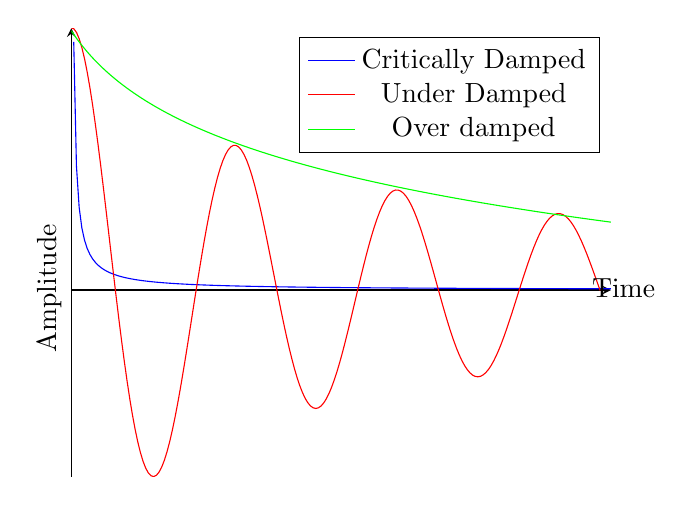
\begin{tikzpicture}
\begin{axis}[axis lines=middle,samples=200,ymax=10,ticks=none,ylabel=Amplitude,ylabel style={rotate=90, anchor=south,at={(axis description cs:0,0.42)},},xlabel=Time,x label style={at={(axis description cs:1.1,0.42)},anchor=east},]
\addplot[blue,domain=0:21] {1/x};\addlegendentry{Critically Damped}
\addplot[red,domain=0.01:20.58] {78*sin(deg(x+7.7))/(x+7.7)};\addlegendentry{Under Damped}
\addplot[green,domain=0.01:21] {-3*ln(x+2)+12};\addlegendentry{Over damped}
\end{axis}
\end{tikzpicture}
\subsection{Forced vibrations and resonance}
\textbf{Free vibrations} - Vibrations where there is no damping and no periodic force acting on the system, amplitude of the oscillations is constant\\
\textbf{Forced vibrations} - Vibrations of a system subjected to an external periodic force
\subsubsection{The effects of damping on the sharpness of resonance}
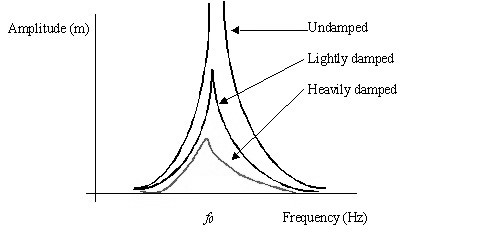
\includegraphics[width=8cm]{damp_6.jpg}\\
The less damping there is, the sharper the resonance
\subsubsection{Standing waves}
Standing waves can be produced at the resonant (natural) frequencies of a material, causing point on it to alternate between minimum and maximum amplitude, causing solid materials such as concrete to break.

\end{document}